\documentclass[a4paper,oneside]{article}

\usepackage{graphicx}
\usepackage{url}
\usepackage{fancyhdr} 
\pagestyle{fancy}


\usepackage{listings}
\usepackage{courier}
\lstset{
         basicstyle=\footnotesize\ttfamily, % Standardschrift
         %numbers=left,               % Ort der Zeilennummern
         numberstyle=\tiny,          % Stil der Zeilennummern
         %stepnumber=2,               % Abstand zwischen den Zeilennummern
         numbersep=5pt,              % Abstand der Nummern zum Text
         tabsize=2,                  % Groesse von Tabs
         extendedchars=true,         %
         breaklines=true,            % Zeilen werden Umgebrochen
         keywordstyle=\color{red},
    		frame=b,         
 %        keywordstyle=[1]\textbf,    % Stil der Keywords
 %        keywordstyle=[2]\textbf,    %
 %        keywordstyle=[3]\textbf,    %
 %        keywordstyle=[4]\textbf,   \sqrt{\sqrt{}} %
         stringstyle=\color{white}\ttfamily, % Farbe der String
         showspaces=false,           % Leerzeichen anzeigen ?
         showtabs=false,             % Tabs anzeigen ?
         xleftmargin=17pt,
         framexleftmargin=17pt,
         framexrightmargin=5pt,
         framexbottommargin=4pt,
         %backgroundcolor=\color{lightgray},
         showstringspaces=false      % Leerzeichen in Strings anzeigen ?        
}
\lstloadlanguages{C}
% Check Dokumentation for further languages ...
         %[Visual]Basic
         %Pascal
%          C
         %C++
         %XML
         %HTML
         %Java
% }
%\DeclareCaptionFont{blue}{\color{blue}} 

%\captionsetup[lstlisting]{singlelinecheck=false, labelfont={blue}, textfont={blue}}
\usepackage{caption}
\DeclareCaptionFont{white}{\color{white}}
\DeclareCaptionFormat{listing}{\colorbox[cmyk]{0.43, 0.35, 0.35,0.01}{\parbox{\textwidth}{\hspace{15pt}#1#2#3}}}
\captionsetup[lstlisting]{format=listing,labelfont=white,textfont=white, singlelinecheck=false, margin=0pt, font={bf,footnotesize}}



\bibliographystyle{unsrt} 
\newenvironment{mylisting}
{\begin{list}{}{\setlength{\leftmargin}{1em}}\item\scriptsize\bfseries}
{\end{list}}
\newenvironment{mytinylisting}
{\begin{list}{}{\setlength{\leftmargin}{1em}}\item\tiny\bfseries}
{\end{list}}


\title{Tutorial:\\Rare Event Sampling with FRESHS and FFS\\using the example of\\polymer translocation through a nanopore simulated with ESPResSo}
\author{Kai Kratzer, Joshua T. Berryman and Axel Arnold}


\begin{document}
\lhead{Rare Event Sampling with FRESHS and ESPResSo}
\rhead{
\includegraphics[height=0.06\linewidth]{pics/freshs-logo.png}\quad 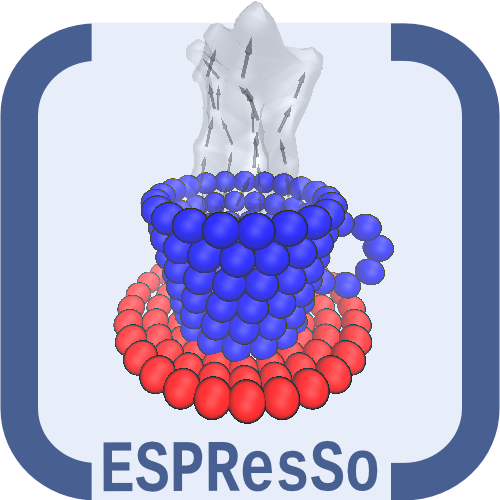
\includegraphics[height=0.06\linewidth]{pics/cup.png}}
% \lfoot{Kratzer, Berryman, Arnold}

\maketitle
\tableofcontents

\newpage

% ----------------------------------------------------------------------------
\section{Introduction and background}

In this tutorial, we present the software package FRESHS~\cite{freshs} for parallel simulation of rare events using sampling techniques from the `splitting' family of methods which are suited to simulate equilibrium and non-equilibrium systems.
FRESHS provides a plugin system for software implementing the underlying physics of the system of interest. At present, example plugins exist for our framework to steer the popular MD packages GROMACS, LAMMPS and ESPResSo, but due to the simple interface of our plugin system, it is also easy to attach other simulation software or self-written code. Use of our framework does not require recompilation of the simulation program.

System states are managed using standard database technology\footnote{Here, we use sqlite3 databases.} so as to allow checkpointing, scaling and flexible analysis.
The communication within the framework uses standard TCP/IP networking and is therefore suited to high-performance parallel hardware as well as to distributed or even heterogeneous networks of inexpensive machines. 
For FFS we implemented an automatic interface placement~\cite{optiflux} that ensures optimal, nearly constant flux through the interfaces.
We introduce `ghost' (or `look-ahead') runs that remedy the bottleneck which occurs when progressing to the next interface.

FRESHS is open-source, providing a publicly available parallelized rare-event sampling system.

We focus now on the FFS simulation technique, which we use here to simulate the polymer translocation through a nanopore.

\subsection{Forward Flux Sampling (FFS)}

FFS is designed to sample the transition rate $k_{AB}$ and transition trajectories from an initial state $A$ to a final state $B$. The transition rate is split into two contributions $k_{AB} = \Phi P_B $, where $\Phi$ is the so-called {\em escape flux}, the flux of trajectories leaving the initial state $A$, and $P_B$ is the probability that a trajectory that manages to leave the initial state $A$ arrives at the final state $B$, instead of returning to $A$.

\begin{figure}
\begin{center}
 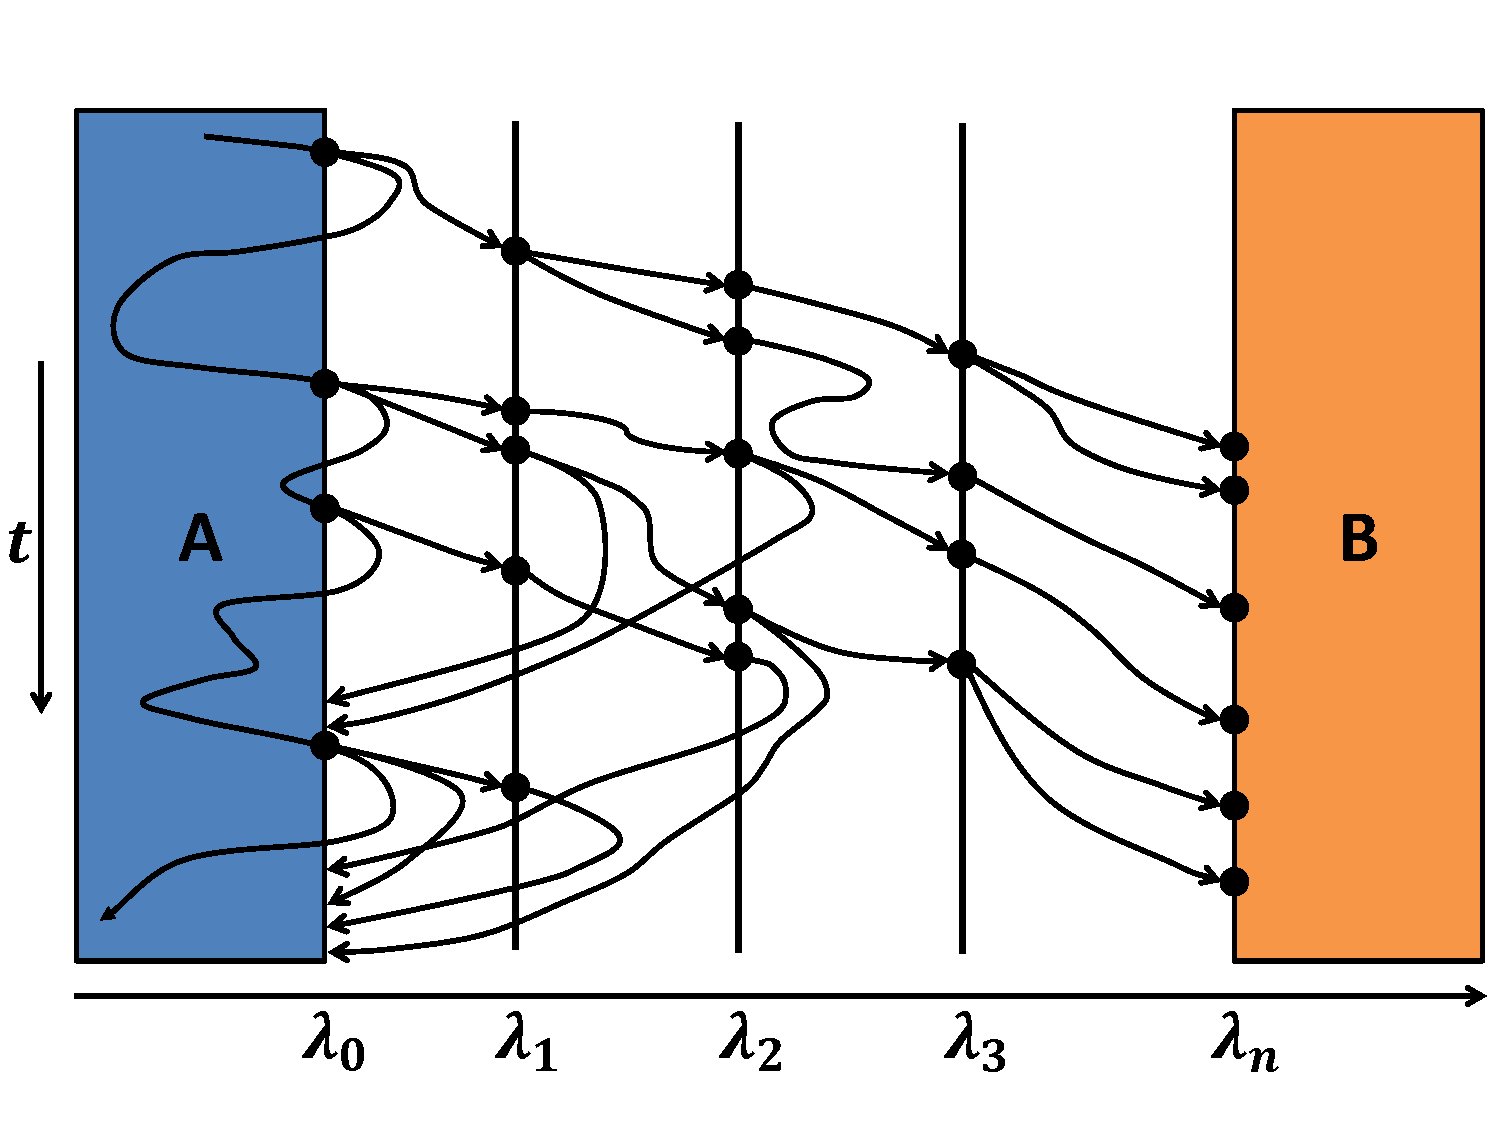
\includegraphics[width=0.7\linewidth]{pics/ffs_plain}
 \caption{Schematic illustration of the FFS algorithm. The ``barrier'' region between the initial state $A$ and the final state $B$ is partitioned by a set of interfaces. The initial MD run in A is used to determine the {\em escape flux} $\Phi$, the other lines depict the successful and the unsuccessful runs which are used to determine $P_B$. The dots represent configurations on the particular interface.
 \label{fig:ffs_hyper}}
\end{center}
\end{figure}

The initial and final states are defined in terms of an order parameter $\lambda$. If $\lambda <= \lambda_A$, the system is in the initial state, if $\lambda_A < \lambda < \lambda_B$, it is in the ``barrier'' region, and if $\lambda > \lambda_B$, the system is in the final state.

Usually, $A$ is defined such that its boundary is still relatively frequently visited, so that $\Phi$ can be determined from a conventional brute-force simulation. $P_B$ however is usually very small and therefore cannot be sampled directly. Therefore, the ``barrier'' region is partitioned by a set of $n$ interfaces $\lambda_i$, where $\lambda_i < \lambda_{i+1}$ and $\lambda_0 \equiv \lambda_A$ and $\lambda_n \equiv \lambda_B$ (fig.~\ref{fig:ffs_hyper}).
The probability $P_B$ is then given by
\begin{equation}\label{eq:ppi}
P_B = \prod_{i=0}^{n-1}p_i
\end{equation}
where $p_i$ is the probability to reach interface $i+1$ coming from interface $i$, before returning back to $A$. The advantage of this splitting is that the probabilities $p_i$ are much higher than $P_B$ itself, and therefore easier to sample. By tracking back the transition paths from interface to interface, FFS also generates transition trajectories, which can be used for investigations of the transition process.

An implementation of the DFFS algorithm consists of two stages. First, the flux $\Phi$ across the first interface $\lambda_0$ is computed by setting up the system in the initial state and monitoring the frequency of trajectory crossings on $\lambda_0$. On occurence of such a crossing, the configuration of the system is stored if the crossing happened in the direction of increasing $\lambda$. This generates $N_0$ configurations corresponding to states of the system at $\lambda_0$. If the system reaches the final state during this run, it is reset to the initial state and re-equilibrated.

In the second stage of the DFFS algorithm, the partial probabilities $p_i$ are computed step-by-step (fig.~\ref{fig:ffs_hyper}). To compute $p_1$, one chooses configurations at random from the configurations stored at the first interface $\lambda_0$  and uses them to fire new "trial" trajectories. These new trajectories are continued until they reach either the next interface $\lambda_1$ or return to the previous interface $\lambda_0$. Again, the successful configurations at $\lambda_1$ are stored in a new set. After $M_0$ trial runs have been fired, $p_1$ is computed by dividing the number of successful runs by $M_0$.  This procedure is repeated using the configurations at $\lambda_1$ as starting points for $M_1$ trial runs that are continued until they reach the next interface $\lambda_2$ or return to $\lambda_0$, and so on, until the final interface at $\lambda_B$ is reached. This procedure results in a complete set of estimated partial probabilities $p_i$. Transition trajectories from the initial 
state $A$ to the final state $B$ can then be reconstructed from the collection of successful trajectories between the two states. For further information, refer to~\cite{fFFS,FFSAllen,efficiency,ffs,barrier}.


\subsection{Polymer translocation through a nanopore}

In this tutorial, we will use the software package ESPResSo~\cite{espresso} together with the Forward Flux Sampling method using ghost runs and automatic, optimized interface placement~\cite{optiflux} to push a polymer through a nanopore (see also fig.~\ref{fig:nanopore}).
\begin{figure}[tb]
 \centering
 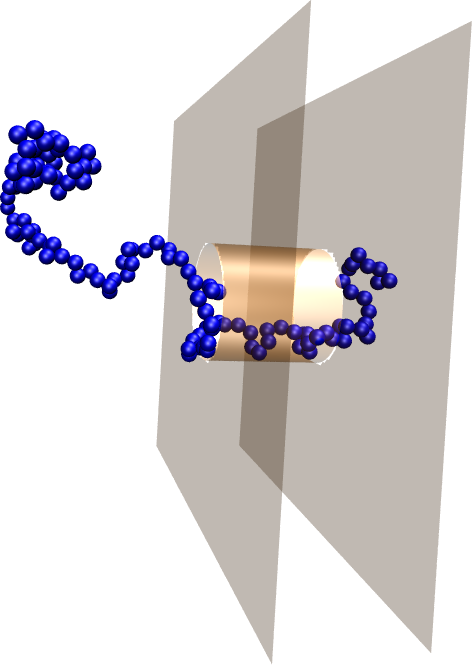
\includegraphics[width=0.3\linewidth]{pics/translocation2}
 \caption{Polymer in a nanopore, set up and simulated using ESPResSo and visualized with VMD.}
 \label{fig:nanopore}
\end{figure}

\subsubsection{Reaction coordinate}\label{sec:rc}
As reaction coordinate, we use the $z$ coordinate in direction of the pore of the center of mass of the polymer chain,
\begin{equation}
 \lambda=\frac{1}{N}\sum_{i=0}^{N-1}z_i,
\label{eq:rc}
\end{equation}
where $N$ is the number of monomers in the polymer chain. Note, that this is probably not the best reaction coordinate, but an easy one which increases in direction to the final state B. As an advanced task you could think about other reaction coordinates and try to implement them.

\subsubsection{Initial state A}\label{sec:initA}
For the setup in the initial state A, we set up a polymer with the first bead located at the entry of the pore. The rest of the polymer is set at random, using the capabilities of ESPResSo to set up random polymers. Then, we check the reaction coordinate. If it is in our basin of state A, we begin the initial MD run in A, if not, we delete the polymer and set a new one.

\subsubsection{Final state B}\label{sec:arrivedB}
The final state is located at a position $\lambda_B$, where most of the polymer has translocated through the pore. This is the case, when the reaction coordinate is larger than the $z$-coordinate of the center of the pore. To make sure, that we are really through, we set the border of state B a little bit behind. 
% If the polymer has passed the top of the energy barrier (has passed the middle of the pore), the probability to go further through should be more than $0.5$.

\subsubsection{Simulation scenario}
For this simulation, we use a box with dimensions $30\times30\times60$ and periodic boundary conditions. The pore's center is in the middle of the box, with a length of $l=10.0$ in $z$-direction. The diameter of the pore can be specific in the configuration file (see sec.~\ref{sec:configfiles}), this is advantageous to investigate the effect of different radii of the pore. We recommend to start with a larger radius at the beginning, e.g. $r=5$. The entry of the pore is located at $\lambda=25$ and the center of the pore is at $\lambda=30$. This means, the polymer is through the pore, when the reaction coordinate is larger than $\lambda=30$. For the border of the initial domain A we choose $\lambda_A=17$, which should be at the beginning of the increase of the free energy curve towards the entry of the pore. 

The number of steps of an initial MD run is limited. However, if the polymer diffuses too much away from the pore, we have to interrupt the simulation before the center of mass is at the other side of the simulation box because of the periodic boundary conditions. Therefore, we initialize our system again in A, if the center of mass is lower than e.g. $\lambda=5$.

The length of the polymer can also be tuned in the configuration file. We start with a shorter polymer, e.g. $N=32$. The polymer uses FENE interactions for the bonds. The other interactions (e.g. polymer-pore) are set to Weeks-Chandler-Andersen interactions.

Now, we proceed with the software requirements and the setup of the environment.


% ----------------------------------------------------------------------------
\section{Requirements}

To follow this tutorial you will need:

\begin{enumerate}
\item A POSIX-compatible operating system (e.g. Linux, Mac OS X)
\item GIT\footnote{\url{http://git-scm.com/}}: Version control system to checkout the latest code
\item FRESHS\footnote{\url{http://www.freshs.org}}: The Flexible Rare Event Sampling Harness System
\item ESPResSo\footnote{\url{http://espressomd.org}}: MD simulation tool which we will couple to FRESHS
\item Python with sqlite support and numpy to execute the code and analysis tools
\item Gnuplot\footnote{\url{http://www.gnuplot.info/}}: Plotting tool for visualizations
\item SQL viewer (optional), e.g. SQLite Manager addon for firefox\footnote{\url{https://code.google.com/p/sqlite-manager/}} or sqlitebrowser\footnote{\url{http://sqlitebrowser.sourceforge.net/}}
\item VMD\footnote{\url{http://www.ks.uiuc.edu/Research/vmd/}} (optional) 
\end{enumerate}

Some package dependencies for a typical unix system might include:

\begin{enumerate}
\item {\bf For ESPResSo:} tcl-dev, automake, libtool, g++
\item {\bf For FRESHS itself:} libsqlite3, numpy
\item {\bf General:} csh (may be needed by vmd), texlive \& bibtex (may be used to build documentation) 
\end{enumerate}



% ----------------------------------------------------------------------------
\section{Preparing the environment}

In this section we will get the required tools and prepare the directory structure, configuration files and simulation tools.

\subsection{ESPResSo}
Checkout the latest ESPResSo code (alternatively, you can use your already existing code snapshot):
\begin{mylisting}
\begin{verbatim}
git clone git://github.com/espressomd/espresso.git
\end{verbatim}
\end{mylisting}

Once you have cloned the development code, to switch to a release that is known to work (e.g. 3.2.0), rather than the latest one, you might want to try:

\begin{mylisting}
\begin{verbatim}
cd espresso
git checkout tags/3.2.0
\end{verbatim}
\end{mylisting}



Make sure that you have the following enabled in your myconfig.hpp:
\begin{lstlisting}
#define CONSTRAINTS
#define LENNARD_JONES
\end{lstlisting}
Compile ESPResSo with these settings and note down the absolute path, where your `Espresso' executable is located. You will need that information later in the client's configuration file.


\subsection{Getting FRESHS and the tutorial files}

The recommended way is to checkout the latest FRESHS development code from github:
\begin{mylisting}
\begin{verbatim}
git clone https://github.com/freshs/freshs.git
\end{verbatim}
\end{mylisting}


Alternatively, you can also download the a release .tar.bz2-package from the webpage, but the development code should have the latest updates included.


After checking out the code from github, several subdirectories should be located in the freshs-directory, here is an overview:
\begin{itemize}
 \item client: The code of the client which connects to the server and launches the harness scripts and the simulation tool.
 \item doc: Documentation of the framework.
 \item harnesses: Example harness scripts.
 \item scripts: Analysis scripts to analyze data during and after the simulation. These scripts can also serve as templates for own analysis scripts.
 \item server: The code of the server which implements all methods and distributes jobs to the simulation clients.
 \item test: Directory containing some test codes. Not used in this tutorial.
 \item tutorial: The tutorial files.
\end{itemize}

% ----------------------------------------------------------------------------
\subsection{Preparing the configuration files}\label{sec:configfiles}
\subsubsection{Server}
Navigate to the `server' folder of the `freshs' directory. Copy the ffs example configuration file to a new configuration file for our simulation:
\begin{mylisting}
\begin{verbatim}
cp server-sample-ffs.conf server-espresso-ffs_tutorial.conf
\end{verbatim}
\end{mylisting}
Open the file with an editor of your choice and change the following sections:
\begin{mylisting}
\begin{verbatim}
[general]
# Change this to something individual (do not use 42, 1337, ...), 
# should be above 1000 and less than 65535
listenport = 
...
# turn on ghosts
use_ghosts = 1
...
# adapt user_msg for easy configuration of the data directory, 
# pore diameter and polymer length.
# Think about a directory, where the snapshots can be stored
user_msg = "servername": "polytranslocsrv", "storedir": 
"/insert/path/to/data/directory", "p_length": 32, "pore_rad": 5

[ffs_control]
# enable parallel escape runs
parallel_escape = 1
...
# use 100000 integration steps for each MD escape trace
escape_steps = 100000

[auto_interfaces]
# use automatic interface placement
auto_interfaces = 1
# minimal distance between interfaces
auto_mindist = 0.001
# maximum number of calculation steps for exploring runs
auto_max_steps = 100000
# minimum acceptable estimated flux
auto_flux_min = 0.4
# maximum acceptable estimated flux
auto_flux_max = 0.6
# use exploring scouts method. Clients must support this.
auto_histo = 1

[hypersurfaces]
# borderA = lambda_A = lambda_0
borderA = 17.0
# borderB = lambda_B = lambda_n
borderB = 33.0

[runs_per_interface]
# borderA = lambda_A = lambda_0
borderA = 200
# borderB = lambda_B = lambda_n
borderB = 100
\end{verbatim}
\end{mylisting}


\subsubsection{Client}
Navigate to the `client' folder of the `freshs' directory. Copy the client example configuration file to a new configuration file for our simulation:
\begin{mylisting}
\begin{verbatim}
cp client-sample.conf client-espresso-ffs_tutorial.conf
\end{verbatim}
\end{mylisting}
Open the file with an editor of your choice and change the following sections:
\begin{mylisting}
\begin{verbatim}
[general]
# the host to connect to, if you only use your machine, set this to localhost
host = localhost
# port of the server which you entered in the server's config
port = 
...
# the path to the Espresso executable (no quotes, absolute path!)
executable = /home/myusername/espresso/Espresso
# location of the harness dir where the 'job_script' is located (no quotes!)
# (will be created in the next section)
harness = ../harnesses/espresso-ffs_tutorial
...
# set unix niceness to 19 to not disturb other processes...
nice_job = 19

[ffs_control]
# ESPResSo is capable of checking the order parameter
checking_script = 1
\end{verbatim}
\end{mylisting}


\subsection{Preparing the harness script}

Espresso scripts are typically written in TCL (``Tool Control Language'').  This is a scripting language that offers the usual constructs of loops, function definitions and so on.  TCL is partly {\bf whitespace sensitive} so take care not to break the layout of the script, eg.: 
\begin{mylisting}
\begin{verbatim}
if { $a == 1 } then 
{ puts "It's true what they say, a really is equal to 1"}
\end{verbatim}
\end{mylisting}

Will not work. The correct format is:
\begin{mylisting}
\begin{verbatim}
if { $a == 1 } then { 
  puts "It's true what they say, a really is equal to 1"
}
\end{verbatim}
\end{mylisting}

or if you want: \verb+if { $a == 1 }{puts "This works too"}+.




The harness script for this tutorial is based on the espresso\_plain example from the harness directory and is located at
\begin{mylisting}
\begin{verbatim}
harnesses/espresso-ffs_tutorial
\end{verbatim}
\end{mylisting}
Open the file job\_script and get a general idea what this script does (the comments in the file should help a lot). Then, look for comments containing a `TODO' and fix the particular parts. Hints:
\begin{itemize}
 \item calc\_rc: \verb+[lindex [part <$id>] 4]+
gives the z-coordinate of the particle with index id. Alternatively, you could have a look in the Espresso user's guide, at the \verb+analyze centermass+ command.
 \item The command to add something to a TCL list is `lappend'.
\end{itemize}
The harness script contains sections to visualize the polymer using VMD. Therefore, VMD must be installed. However, this is only reasonable for the first run, to ensure that the system is set up correctly. For the productive run, this sections should be commented, you'll see why when you start the client.


% ----------------------------------------------------------------------------
\section{Launching FRESHS}

FRESHS consists of two separate python programs, the {\it server} and the {\it client}.  Parallelism is achieved by running multiple copies of the client; which are controlled centrally by the server. In addition, ESPResSo can calculate the physics in parallel, too. Note, that this makes only sense for larger systems, not for a polymer of $32$ beads like in our example. Here, it should be faster to use multiple clients.

Open a new terminal, navigate to the server directory and start the server with
\begin{mylisting}
\begin{verbatim}
python main_server.py -c server-espresso-ffs_tutorial.conf
\end{verbatim}
\end{mylisting}
This should start the server which listens now on the specified port. Open a new terminal (or a new tab in the current session for better overview), navigate to the client directory and start a client using
\begin{mylisting}
\begin{verbatim}
python main_client.py -c client-espresso-ffs_tutorial.conf
\end{verbatim}
\end{mylisting}
which starts a client connecting to the server.

If things aren't working, then check the error messages and make sure that you set the right paths to the harness and to the various executables.  If things are hanging you can e.g. kill all clients using the following command:
\begin{mylisting}
\begin{verbatim}
kill `ps -ef | grep main_client.py | grep client-espresso-ffs | awk '{print $2}'`
\end{verbatim}
\end{mylisting}

If everything is running, have a look at the command line output of the server and if you see numbers counting up, lean back and relax, grab a coffee or go to the toilet. Then proceed with the next section.

\section{Analysis tools}

FRESHS saves a comprehensive description of everything it has done into an SQL database, which by default goes into the directory `DB'.  This database is deeply informative, but is not immediately readable, so a number of scripts are provided to construct graphs based on the information within. At the end of a simulation, a summary of the simulation is printed and the interface information and transition rates are saved in the `OUTPUT' directory. In addition to that, several post-processing tools which read out the database can be applied.

\subsection{Database view}
If you have the `sqlitebrowser' or the firefox `SQLite Manager' plugin installed, then use them to have a look at the raw data which comprises the output database, really it is just a big table of simulation information with one row for each trajectory fragment (fig.~\ref{fig:sqlitemanager}), which contains the state at the end of the fragment, as well as enough information to re-generate it (i.e.~a pointer to the parent fragment, and an RNG seed).
\begin{figure}
 \centering
 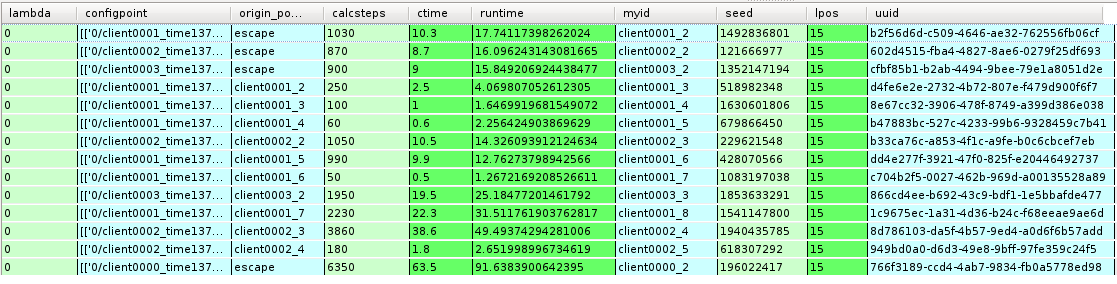
\includegraphics[width=0.99\linewidth]{pics/freshs-sqlite-view}
 \caption{View of the database with SQLite Manager.}
 \label{fig:sqlitemanager}
\end{figure}
The database can be already analyzed and viewed during the simulation. Note, that you should not write to the database during the simulation, handle with care. If the simulation fails at a certain stage, data can be modified/deleted, and the simulation can be resumed from the last state in the database using the `-r' flag of the server.

\subsection{Analysis scripts}
The folder `scripts' in your FRESHS directory contains analysis scripts which can be used directly to e.g. backtrack successful runs or to serve as templates for own analysis scripts.

\subsubsection{Backtracking successful runs}
Change to the `scripts' folder and run the following script:
\begin{mylisting}
\begin{verbatim}
./ffs_buildTree_success.py ../server/DB/<timestamp>_configpoints.sqlite
\end{verbatim}
\end{mylisting}
The output is written to a folder called `OUTPUT/timestamp'. Change to this directory, start gnuplot and plot the tree graph to visualize the traces which lead to the points on the last known interface (fig.~\ref{fig:traces}):
\begin{mylisting}
\begin{verbatim}
load "tree_success.gnuplot"
\end{verbatim}
\end{mylisting}

\begin{figure}
 \centering
 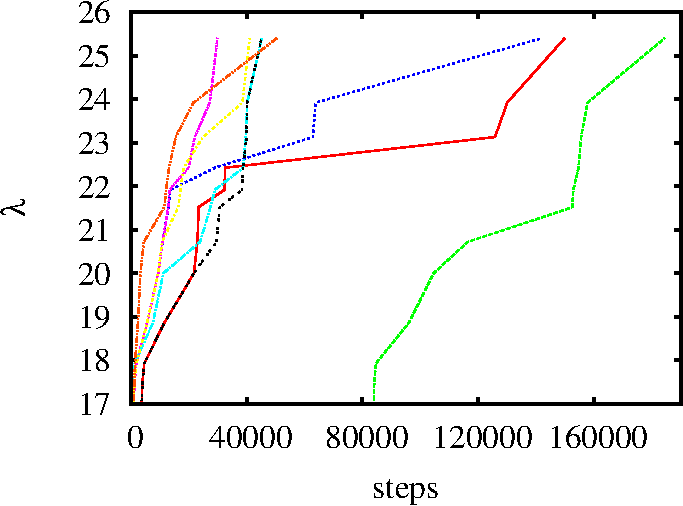
\includegraphics[width=0.5\linewidth]{pics/traces}
 \caption{Backtracking successful runs is already possible during the simulation. Then, the runs are backtracked from the last known interface.}
 \label{fig:traces}
\end{figure}

\subsubsection{Interface statistics}
To plot statistical information about the simulation, e.g. a histogram of the runtime of the clients or a histogram of the calculation steps, run
\begin{mylisting}
\begin{verbatim}
./ffs_interfaces_statistics.py ../server/DB/<timestamp>_configpoints.sqlite
\end{verbatim}
\end{mylisting}
The output is written again to the folder called `OUTPUT/timestamp'. Change to this directory, start gnuplot and plot the histograms:
\begin{mylisting}
\begin{verbatim}
load "histo_runtime.gnuplot"
load "histo_calcsteps.gnuplot"
\end{verbatim}
\end{mylisting}


\subsubsection{Analyzing custom data}
Use the template `scripts/ffs\_customdata.py' to write a script which plots the reaction coordinate distribution from the field `customdata' of the database for each interface. This can already be applied when the simulation is still running like the analysis examples before.
\begin{mylisting}
\begin{verbatim}
#!/usr/bin/python

import sys
sys.path.append('../server/modules')
sys.path.append('../server/modules/ffs')

# custom
import configpoints

def extract_customdata(interface,dbhandle):
    customdata = dbhandle.return_customdata(interface)
    floatdata = []
    for el in customdata:
        for el2 in el.split():
            floatdata.append(float(el2))
    return floatdata

if len(sys.argv) < 2:
    print "Usage:", sys.argv[0], "<../server/DB/configpoint-DB-file>"
    exit(1)

cfph = configpoints.configpoints('none', sys.argv[1])

maxlam = cfph.biggest_lambda()

for i in range(maxlam+1):

    print "Interface", i
    print extract_customdata(i,cfph)
    # TODO: build histograms
\end{verbatim}
\end{mylisting}

\section{FAQ and troubleshooting}
\begin{itemize}
 \item Clients do not find the executable:\\
  Please give the absolute path to the executable and check, that it has the right permissions.
 \item Killing clients:\\
Sometimes, clients launched in a thread can not be killed by pressing CTRL+C. Therefore, it is useful to use e.g.
\begin{mylisting}
\begin{verbatim}
kill `ps -ef | grep main_client.py | grep client-espresso-ffs | awk '{print $2}'`
\end{verbatim}
\end{mylisting}
for killing all the clients which are executed with the espresso-ffs config. Please be careful doing this, you might e.g. first have a look at the output of the ps and grep combination.
 \item Speeding up the server:\\
 If the server's database is located e.g. on a network file system, the access can be slow. Change the location of the database folder in the server's configuration file to a faster location (or create a symbolic link), e.g. a local hard drive (/tmp directory should be always writeable, but remember the size limitation), an SSD or a temporary RAM filesystem (tmpfs).
 \item If a bond of the polymer breaks, consider reducing the timestep of the simulation (and increase the integration steps per cycle accordingly).
\end{itemize}

\begin{thebibliography}{1}

\bibitem{freshs}
K.~Kratzer, J.~T. Berryman, A.~Taudt, and A.~Arnold.
\newblock {The Flexible Rare Event Sampling Harness System (FRESHS)}.
\newblock {\em Submitted}, 2013.

\bibitem{optiflux}
K.~Kratzer, A.~Arnold, and R.~J. Allen.
\newblock Automatic, optimized interface placement in forward flux sampling
  simulations.
\newblock {\em J. Chem. Phys.}, 138(16):164112, 2013.

\bibitem{fFFS}
R.~J. Allen, P.~B. Warren, and P.~R. ten Wolde.
\newblock Sampling rare switching events in biochemical networks.
\newblock {\em Phys. Rev. Lett.}, 94:018104, 2005.

\bibitem{FFSAllen}
Rosalind~J. Allen, Daan Frenkel, and Pieter~Rein ten Wolde.
\newblock Simulating rare events in equilibrium or nonequilibrium stochastic
  systems.
\newblock {\em J. Chem. Phys.}, 124:024102, 2006.

\bibitem{efficiency}
Rosalind~J. Allen, Daan Frenkel, and Pieter~Rein ten Wolde.
\newblock Forward flux sampling-type schemes for simulating rare events:
  Efficiency analysis.
\newblock {\em J. Chem. Phys.}, 124(19):194111, 2006.

\bibitem{ffs}
Rosalind~J Allen, Chantal Valeriani, and Pieter~Rein ten Wolde.
\newblock Forward flux sampling for rare event simulations.
\newblock {\em Journal of Physics: Condensed Matter}, 21(46):463102, 2009.

\bibitem{barrier}
C.~Valeriani, R.~J. Allen, M.~J. Morelli, D.~Frenkel, and P.~R. ten Wolde.
\newblock Computing stationary distributions in equilibrium and nonequilibrium
  systems with forward flux sampling.
\newblock {\em J. Chem. Phys.}, 127:114109, 2007.

\bibitem{espresso}
Bernward A.~Mann Hans-J\"org~Limbach, Axel~Arnold and Christian Holm.
\newblock Espresso -- an extensible simulation package for research on soft
  matter systems.
\newblock {\em Comput. Phys. Commun. 174}, 9:704--727, 2006.

\end{thebibliography}


\end{document}
